\chapter{Estudio del Problema Singular}

En este capitulo se van a aplicar las herramientas desarrolladas en el capitulo anterior al estudio del espectro de un operador singular.

\section{El Operador Singular}

Como trabajo de tesis se propondra aplicar los metodos desarrollados en el capitulo anterior al operador diferencial (\ref{operador}).

\begin{equation}
\begin{array}{c}
    A \phi (x) = - \partial ^2 _x  \phi(x) + \frac{\alpha}{x} \phi(x) \\
    \phi(0) = \phi(L) = 0 
\end{array}
\label{operador}
\end{equation}

Para eso voy a resolver la ecuación de autovalores (\ref{eq.aut.sin}).

\begin{equation}
\begin{array}{c}
    A  \phi (x)  =   \lambda ^2 \phi (x) \\ 
    \lambda \ \in \ \mathfrak{R} _+
\end{array}
\label{eq.aut.sin}
\end{equation}




La cual posee soluciones LI, $ y_1 $ y $ y_2 $ dadas por :

\begin{equation}
    \phi (x) = 
    C[1]
    \underbrace{
     \ e ^{-i \lambda x} \ x \ F _{1} ^{1} (1+\frac{ \alpha}{2 \lambda i },2,2 i \lambda x) } _ {y_1}
    + C[2] \underbrace{ \ e^{-i \lambda x } \ x \ U (1+\frac{ \alpha}{2 \lambda i },2,2 i \lambda x) } _{y_2} 
\end{equation}


%Para autovalor $- \lambda ^2 $ obtengo las siguientes soluciones:

%\begin{equation}
%    \phi ^{-} (x) = 
%    \underbrace{
%    C[1] \ e ^{-i \lambda x} \ x \ F _{1} ^{1} (1 + \frac{ \alpha}{2 \lambda},2,2 i \lambda x) } _ {y_1}
%    + \underbrace{C[2] \ e^{-i \lambda x } \ x \ U (1 + \frac{ \alpha}{2 \lambda},2,2 i \lambda x) } _{y_2} 
%\end{equation}

Donde $F _1 ^1(a,b,z)$ y $ U(a,b,z)$ son las soluciones LI de la ecuacion hypergeometrica (\ref{eq:hyper})

\begin{equation}
    z \ \partial ^2 _z \ \psi (a,b,z) + (b-z) \
    \partial _z \psi (a,b,z)
    -a \ \psi (a,b,z) = 0
\label{eq:hyper}
\end{equation}

Las cuales tienen las siguientes expresiones analiticas  : 

\begin{equation}
\begin{array}{c}
	U(a,b,z) = \frac{1}{\Gamma (a)} 
	\int _0 ^{\infty} e ^{-zt}
	t ^{a-1}
	(1+t) ^{b-a-1}
	dt \\
	F _1 ^1 (a,b,z) = \sum _ {k=0} ^{\infty} 
	\frac{(a) _k}{(b) _k} 
	\frac{z ^k}{k!} 
\end{array}
\end{equation}

%\textbf{Estados Ligados:} \\

%Primero voy a buscar estados ligados, imponiendo la condicion $\phi ^{-} (0) = 0$, veo que $U(1- \frac{\alpha}{2 \lambda} ,2 ,0) \rightarrow \infty $ obtengo $C[2] = 0$

%Los estados ligados van a surgir entonces de la condicion de contorno en $x=L$

%\begin{equation}
%	F _1 ^{1} (1- \frac{\alpha}{2 \lambda} , 2 2 i \lambda L ) = L 
%\end{equation}


\textbf{Espectro del operador:} \\
%    A partir de aquí $\phi ^{+} (x)$ la escribiré $\phi (x)$ \\


Para aplicar la condicion de contorno $\phi (0) = 0$, hay que hacer un desarrollo de $\phi(x)$  alrededor de $x \rightarrow 0$:

\begin{equation}
\begin{array}{c}
\phi (x \rightarrow 0) \approx
C[1] ( x + O(x ^2)) + 
C[2] x 
\left( 
\frac{1}{  \alpha x  \Gamma ( \frac{ \alpha}{2 i \lambda}  )   }  +
\frac{Log(x) }{\Gamma ( \frac{ \alpha}{2 i \lambda} ) } + Cte + O(x)
\right)
\\ \\
Donde,  \ Cte = 
\frac{
-1 + 2 \gamma + Log[2 i \lambda] + \psi (1 + \frac{ \alpha}{2 i \lambda})
}
{\Gamma (\frac{i \alpha}{2 \lambda})}
\end{array}
\label{eq.scat}
\end{equation}

Donde se ve que $y _1 (x \rightarrow 0 ) \rightarrow 0$ y $y _2 (x \rightarrow 0)  \rightarrow
\frac{1}{  \alpha   \Gamma ( \frac{i \alpha}{2 \lambda}  )   } $ , entonces la forma de satisfacer la condicion de contorno es imponiendo C[2] = 0

Los autovalores estaran dados entonces por los ceros de $y_1 (x= L)$, como el único termino que se anula en el produco es la funcion Hypergeometrica, los autovalores vienen dados por los ceros de la ecuacion (\ref{eq.1}), en la figura (\ref{fig:funcion}) en funcion de $\lambda$ para  $\alpha=1, \ L=1$.:


\begin{equation}
F _1 ^1 (1+\frac{ \alpha}{2 i \lambda},2,2 i \lambda L)  = 0
\label{eq.1}
\end{equation}

\begin{figure}
\centering
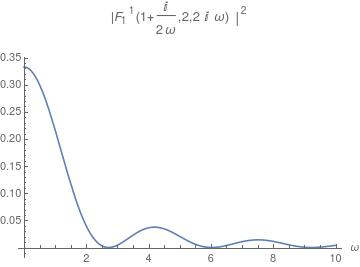
\includegraphics[scale=0.7]{Funcion.jpg}
\caption{En esta imagen se puede ver el comportamiento de los ceros de función $F _1 ^1$, para $\alpha=1$ y $L=1$}
\label{fig:funcion}
\end{figure}

\textbf{Desarrollo en serie:} \\

Para estudiar el espectro de $F _1 ^1$ voy a hacer un desarrollo asintotico alrededor de $\lambda \rightarrow \infty$, el cual está dado por (\ref{eq.aprox})


\begin{equation}
\begin{array}{c}
    F _1 ^1 (a,b,z) = \Gamma (b) 
    \left(
    \frac{e^z z ^{a-b} }{\Gamma(a)} * S_1 + \frac{(-z) ^{ -a}}{ \Gamma(b-a)} 
    * S_2
    \right) \\ 
    S _1 = \sum _{n=0} ^{\infty} \frac{(b-a) _n (1-a) _n}{n!} z ^{-n} \\ 
    S _2 = \sum _{n=0} ^{\infty} \frac{(a) _n (1+a-b) _n}{n!} (-z) ^{-n}
    
\end{array}
\label{eq.aprox}
\end{equation}

$A_1$ y $A _2$ son las correcciones al orden domintante, para calcular el polo de la funcion $\zeta _A (s)$ en $s=-1/2$ basta tomar $A _1 = A _2 = 1$, que es lo que se hará, luego se trabajará con el desarrollo en serie completo para estudiar los polos mas allá de $s=-1/2$. 

%Donde $A_1$ y $A_2$ son los demas terminos de la serie, que voy a tomar como 1, en el apéndice 1 voy a demostrar que no contribuyen a la estructura de los polos al orden que estoy calculando, si hay que tenerlos en cuenta para calcular los polos mas halla de donde se calcularon en esta tesis.

Quedandome solo con el orden domintante obtengo para la ecuacion (\ref{eq.aprox}) %, definiendo las variables adimensionales $\mu = \lambda L$, $\beta = \alpha L $, obtengo para la ecuación  (\ref{eq.aprox}):. 

\begin{equation}
    F _1 ^1 (1+  \frac{  \alpha}{2 i \lambda} ,2 ,2 i \lambda L  ) = 
   i  \frac{e ^{ \frac{\pi}{4} \frac{\alpha}{\lambda} } }{2 \lambda L}
    \left( -
    \frac{e ^{- i \frac{\alpha}{2 \lambda} Ln(2 \lambda L) } e ^{2 i \lambda L} }{\Gamma(1+\frac{ \alpha}{2 i \lambda})} +
    \frac{e ^{  i \frac{\alpha}{2 \lambda} Ln(2 \lambda L) }}               {\Gamma(1-\frac{ \alpha}{2 i \lambda})}
    \right)
\label{eq.completa}
\end{equation}




La cual queda expresada como un producto de dos funciones, una parte que se anula y una parte que no.

Para obtener los autovalores voy a solo ocuparme de la parte que se anula, la cual esta entre paréntesis.

\begin{equation}
    M (\mu) = 
    - \frac{e ^{- i \frac{\alpha}{2 \lambda} Ln(2 \lambda L) } e ^{2 i \lambda L} }{\Gamma(1+\frac{ \alpha}{2 i \lambda})} +
    \frac{e ^{  i \frac{\alpha}{2 \lambda} Ln(2 \lambda L) }}               {\Gamma(1-\frac{ \alpha}{2 i \lambda})}
\label{eq.aproxx}
\end{equation}

Para el calculo de la funcion $\zeta _A (s) $ se puede utilizar $M ( \mu )$ o cualquier multiplo de ella, ya que posee los mismos autovalores que $F_1 ^1 $

%En todas las cuentas posteriores, para calcular $\zeta _A (s)$ voy a utilizar $M ( \mu )$ ya que posee los mismos autovalores de $ F _1 ^1 $.



\section{Calculo Asintótico de los autovalores}


En está seccion voy a definir las variables adimensionales $\mu = \lambda L $ y $\beta = \alpha L$.

Entonces el problema queda determinado por conocer los ceros $\mu _n$ de $M(\mu)$, a $\mu _n \rightarrow{\infty}$, suponiendo que a $\mu _n$ la puedo descomponer en una parte divergente mas una infinitesimal cuando $n \rightarrow{\infty}$, tal como en el capitulo anterior.


Para que el desarrollo sea mas simple, voy a voy a escribir a $M (\mu)$ como:

\begin{equation}
M (\mu) = e ^{\frac{i \beta Log(2 \mu)}{\mu}}
\frac{\Gamma (1- \frac{i \beta}{2 \mu})}{\Gamma (1 + \frac{i \beta}{2 \mu})}
- e ^{2 i \mu}
\label{eq.otro.mu}
\end{equation}


En el limite de $\mu _n \rightarrow \infty$ se obtiene:

\begin{equation}
    M(\mu _n \rightarrow \infty) = 
	1 - e ^{2 i \mu}
\end{equation}

De acá se puede ver que el comportamiento de $\mu _n$ esta dado por 


\begin{equation}
\begin{array}{c}
    \mu _n = n \pi + \epsilon _n \\
    Donde \ \epsilon _n \rightarrow{0} ,\ si \ n \rightarrow{0}
\end{array}
\label{eq.mu2}
\end{equation}



Para calcular orden a orden el termino $\epsilon _n$ inserto la ecuación (\ref{eq.mu2}) en (\ref{eq.otro.mu}) e igualo la ecuación a cero, lo cual conduce a la siguiente ecuación para $\epsilon _n$

\begin{equation}
	e ^{ i \frac{\beta}{ \mu _n} Ln(2 \mu _n)}     
    \frac{\Gamma(1 - \frac{i \beta}{2  \mu _n} ) }
    {\Gamma(1 +  \frac{i \beta}{2  \mu _n} )} =    
    e ^{2 i \epsilon _n }
\end{equation}

teniendo en cuenta que $\frac{ln(2 \mu _n)}{2 \mu _n }$ tiende a cero a $\mu _n$ grade, puedo hacer un desarrollo de la exponencial y las funciones $\Gamma$ alrededor de $ \mu _n \rightarrow \infty $, y $\epsilon _n \rightarrow 0$

\begin{equation}
    \left(
    \sum _{p = 0} ^{\infty} \frac{ \left( i \frac{\beta}{ \mu} Log(2 \mu ) \right) ^p }{p!}
    \right)
    \left(
	\sum _{q = 0} ^{\infty} \frac{a _q}{\mu ^q}
	\right)
    =
    \left(
    \sum _{l = 0} ^{\infty} \frac{( 2 i \epsilon _n)^l}{l !}
    \right)
\end{equation}


Al orden mas bajo se obtiene la ecuación : 

\begin{equation}
(1 + \frac{i \beta}{ \mu} Log( 2 \mu) ) 
(1 + \frac{i  \gamma \beta}{ \mu})  =
(1 + 2 i \epsilon)
\end{equation}

Todo esto conduce a que el termino subdominante sea $\epsilon _n =  \frac{\beta \ Ln(2 n \pi)}{2 n \pi}$ , pero con esto no alcanza, ya que existe otro termino que decae como 1/n, para calcular el polo en $s=-1/2$ se deben calcular todos los términos que decaigan como 1/n, insertando $\epsilon _n =  \frac{\beta Ln(2 n \pi)}{2 n \pi} + \epsilon '$ en la ecuación anterior, obtengo:


\begin{equation}
    \epsilon _n =  \frac{\beta Ln(2 n \pi)}{2 n \pi} +
                \frac{\gamma \beta}{2 n \pi} +
                O(\frac{1}{n^2})
\end{equation}

Luego para calcular la función $\zeta _{A}$ utilizo su definición

\begin{equation}
\begin{array}{c}
    \zeta _A (s) = \sum _{n=1} ^{\infty} \lambda _n ^{-2 s}  =
    \sum _{n=1} ^{\infty} \left(\frac{\mu _n}{L} \right) ^{-2 s} =  \\
    L ^{2 s} \sum _{n=1} ^{\infty} 
    \left( 
    n \pi + \frac{\beta Ln(2 n \pi)}{2 n \pi} + \frac{\gamma \beta}{2 n \pi} +
    O(\frac{1}{n^2})
    \right) ^{-2s} = \\
    
\end{array}
\end{equation}

Como en el ejemplo anterior puedo escribir todo como:

\begin{equation}
\begin{array}{c}
    \zeta _A (2 s) = \left( \frac{L}{\pi} \right)  ^{2 s} 
    \sum _{n=1} ^{\infty} n ^{- 2  s}
    \left(
    1 + \frac{\beta \ Ln(2 n \pi)}{2 n^2 \pi ^2} + \frac{\gamma \beta}{2 n^2 \pi ^2 } +
    O \left( \frac{1}{n^3} \right)  \right) ^{-2 s} = \\
    ( \frac{L}{\pi} ) ^{2 s}
    \sum _{n=1} ^{\infty} n ^{-2 s} 
    \left(
    1 + \chi _n \right) ^{- 2 s}
\end{array}
\end{equation}

Utilizando como en el ejemplo anterior el desarrollo de la ecuacion para $\chi \rightarrow 0$, donde lo tengo que llevar hasta la potencia $ \chi  $ para sumar todos los terminos que decaigan como $\frac{1}{n ^2}$ (el termino $\chi ^2 $ la potencia mas baja que aporta es $\frac{1}{n ^4}$). La Funcion $\zeta _A (s)$ queda expresada como:


\begin{equation}
\begin{array}{c}
    \zeta _A (s) = ( \frac{L}{\pi} ) ^{2 s}
    \sum _{n=1} ^{\infty} 
    n ^{-2s}
    \left(
    1 - 2 s \chi + O(\chi ^2)
    \right) =  \\
    ( \frac{L}{\pi} ) ^{2 s}
    \left(
    \sum _{n=1} ^{\infty} n ^{-2 s} 
    \left(
    1 - 2s \left(
    \frac{\beta Log[2 n \pi]}{2 n ^2 \pi ^2} + 
    \frac{\gamma \beta}{2 n ^2 \pi ^2} 
	\right) +
    O (\frac{1}{n ^{3} }  )
    \right)
    \right)
\end{array}
\end{equation}


\begin{equation}
\begin{array}{c}
    \zeta _A (s) = 
    \left( \frac{L }{ \pi } \right) ^{2 s}  \\
    \left(
    \zeta (2 s) -
	\frac{ s \beta}{ \pi ^2} \zeta (2s+2)
	\left(
	   Log[2  \pi ] + \gamma
	\right) +
    \frac{s \beta}{\pi ^2}
	\zeta '(2s+2) \
	\right) + \\
    \sum _{n=1} ^{\infty} O \left( \frac{1}{n ^{2s+3}} \right)
\end{array}
\end{equation}

Donde sabiendo que $\zeta(s) = \frac{1}{s-1} + Regular$, el primer polo queda determinado como

\begin{equation}
    \zeta _A (s \rightarrow 1/2) = \frac{L}{2 \pi} \frac{1}{s-1/2}    
\end{equation}

Luego desarrollando alrededor de $s=-1/2$:

\begin{equation}
    \zeta _A (s \rightarrow -1/2 ) =  \frac{\alpha}{8  \pi (s+1/2)^2} +
    \alpha \frac{ \gamma -1 + Log(2L )}{4  \pi (s+1/2)} + 
    Regular
\end{equation}

\section{Calculo Utilizando Variable Compleja}


Sabiendo que los autovalores de mi Hamiltoniano son todos reales, puedo expresar $\zeta _A (s)$ como una integral en el plano complejo, y deformar la trayectoria hasta el camino dado por la figura [\ref{fig:contorno}], tal como se hizo en el capitulo anterior: \\

Mi funcion $ \zeta _A (s) $ va a quedar definida por:

\begin{equation}
\zeta _A (s) = 
\frac{1}{2 \pi i} 
\int _{\mathcal{C}}
\frac{M ' ( z ) }{ M ( z ) } d z
\label{eq.zeta.compleja}
\end{equation}

Donde $M ( z )$ está dada por (\ref{eq.completa}).
cuando integre los ejes verticales, voy a obtener un termino exponencialmente decreciente y uno decreciente, que se van a alternar dependiendo de si estoy arriba o abajo del eje real. \\

Reemplazando la parametrizacion $ z (t) = \pm i t$ en (\ref{eq.zeta.compleja}) y tirando los terminos exponencialmente decrecientes, obtengo:

\begin{comment}

\begin{equation}
\begin{array}{c}
    \zeta _A (s) = \\
     \frac{1}{2 \pi i} \int _{\infty} ^{1}
     \frac{ i \alpha }{2 t^2} 
     \left(
      1 + \frac{i \pi}{2} + Log[2 t] + \psi (1 + \frac{\beta}{2 t})
     \right)
     t ^{-2s}
     e ^{- i \pi s} (i dt) + \\
     \frac{1}{2 \pi i} \int _{\infty} ^{1} 
     \left(
     2 + \frac{\beta}{2 t^2}
     \left(
     1 + \frac{i \pi}{2} - Log[2 t] - \psi (1+ \frac{\beta}{2 t})
     \right)
     t ^{-2s}
     e ^{ i \pi s} (-i dt)
     \right)     
\end{array}
\end{equation}

\end{comment}

\begin{equation}
\begin{array}{c}
    \zeta _A (s) = \\
     \frac{e^{-i \pi s}}{2 \pi i} \int _{\infty} ^{1}
     \frac{ i \alpha}{2 t^2}
     \left(
     - 1 + Log(2 L t) + \frac{i \pi}{2}  - \psi (1+\frac{\alpha}{2 t})
     \right)
     t^{-2 s}
      \ 
     (i dt) + \\
     \frac{e^{i \pi s}}{2 \pi i} \int _1 ^{\infty}
	\left(      
     \frac{ i \alpha}{2  t^2}
     \left(
     1 - Log(2 L t) + \frac{i \pi}{2} + \psi (1 + \frac{\alpha}{2 t}) 
      
     \right)
     + 2 i L
     \right)
     t^{-2 s}
     (-i dt)
     
\end{array}
\end{equation}

Donde antes de reacomodar los terminos puedo calcular el termino que contiene $2iL$ el cual es la potencia mas alta de $t$ para obtener: 

\begin{equation}
    \frac{e^{i \pi s}}{2 \pi i }
    \int _1 ^{\infty}
    2 i L    
    t ^{-2 s}
    (-i dt) =  
    \frac{L e^{i \pi s} }{2 \pi i} \frac{1}{s-1/2   }
\end{equation}

Ningún otro termino aportará a este polo, entonces el polo en $s= 1/2$ es:

\begin{equation}
    \zeta  (s \rightarrow 1/2) = \frac{L}{2 \pi} \frac{1}{s- 1/2 } + Regular
\end{equation}

Que se corresponde con lo calculado con el método anterior. \\

Una vez calculado este termino, puedo reorganizar el resto de la integral como:

\begin{equation}
\begin{array}{c}
    \frac{\alpha}{2 \pi} \ sin(\pi s)
    \int _1 ^{\infty}
    t ^{-2 s-s} 
    \left(
    1 - Log[2Lt] + \psi (1 + \frac{\alpha}{2t})
    \right) dt \ + \\ 
    \frac{\alpha}{4} 
    Cos[\pi s]
    \int _1 ^{\infty} t^{-2s-s} dt
\end{array}
\end{equation}

Donde todos los términos son calculables analíticamente, excepto el que esta multiplicado por $\psi$, para lo cual utilizo el desarrollo de $\psi$ en $t \rightarrow \infty$:

\begin{equation}
    \psi(1 + \frac{\alpha}{2 t}) \approx 
    - \gamma + O \left( \frac{1}{t} \right)
\end{equation}

Realizando todas las integrales, la funcion $ \zeta _A (s)$ a este orden queda determinada por:  

\begin{equation}
\begin{array}{c}
    \zeta (s) _{A} = 
    \frac{L e ^{i \pi s}}{2 \pi i} \frac{1}{s-1/2} 
    -\frac{\alpha Sin(\pi s)}{8 \pi} \frac{1}{(s+1/2) ^2} \\
    + \frac{\alpha sin (\pi s) }{4 \pi } \frac{1 - \gamma -  Log(2 L)}{s+1/2}
    + \frac{\alpha Cos(\pi s)}{8} \frac{1}{s+1/2}
    
\end{array}
\end{equation}

Donde el siguiente termino en el desarrollo de $ \psi $ contribuirá al residuo en $s = -3/2$.

Para calcular el residuo en $s=-1/2$ desarrollo todo en Serie de Laurent obteniendo.

\begin{equation}
	\zeta (s \rightarrow -1/2) = 
     \frac{\alpha}{8 \pi} \frac{1}{(s+1/2)^2} + 
    \alpha \frac{\gamma + Log[2 L] - 1}{4 \pi} \frac{1}{s+1/2} + \ Regular
\label{eq.desarrollo}
\end{equation}

Donde se puede ver que el polo coincide con lo calculado anteriormente. \\

%Una aclaracion importante es que el termino $Log[2 L ]$ es correcto dimensionalmente, ya que proviene de evaluar la integral $\int _1 ^\infty  Log[2 L \lambda] \ d \lambda$

\textbf{Siguientes Polos:} \\

Para calcular los siguientes polos mas allá de $s=-1/2$, voy a volver a calcular la funcion $\zeta _A (s) $ con variable compleja, pero utilizando todos los terminos de la expancion en seríe de la funcion $M ( \lambda )$:

\begin{equation}
\begin{array}{c}
M( \lambda ) = 
 \frac{ e ^{   \frac{i \alpha Log \left(2 \lambda L \right) } 
           {2 \lambda } } }
      { \Gamma \left( 1 + \frac{i \alpha}{2 \lambda}  \right)   } S2 ( \lambda ) -
 \frac{e ^{ - \frac{i \alpha Log \left( 2 \lambda L \right) }{2 \lambda } } e ^{2 i \lambda L } }
      { \Gamma \left( 1 - \frac{i \alpha}{2 \lambda}  \right) } S1 ( \lambda ) \\
      
S1 ( \lambda ) = \sum _{n=0} ^{ \infty }
\frac{\Gamma (1 + \frac{i \alpha}{2 \lambda} + n )}{\Gamma (1 + \frac{i \alpha}{2 \lambda})} 
\frac{\Gamma (\frac{i \alpha}{2 \lambda} + n )}{\Gamma (\frac{i \alpha}{2 \lambda})} 
\frac{1}{( 2 i \lambda L ) ^n} \\

S2 (\lambda ) = \sum _{n=0 } ^{\infty}
\frac{ \Gamma ( 1- \frac{i \alpha}{2 \lambda } + n ) }{\Gamma ( 1- \frac{i \alpha}{2 \lambda } )}
\frac{\Gamma (- \frac{i \alpha }{2 \lambda} + n )}{\Gamma (- \frac{i \alpha }{2 \lambda} )}
\frac{1}{( - 2 i \lambda L ) ^n}
\end{array}
\end{equation}

Donde $S1 (\lambda ) $ y $S2 (\lambda)$ son series de potencias negativas.  \\

Al igual que antes, cuando integre sobre los ejes verticales voy a tener una parte exponencialmente creciente/decreciente, tirando estos terminos los logaritmos quedan (salvo constantes aditivas):

\begin{equation}
\begin{array}{c}

Log ( M ( \lambda = i t ) ) =  Log(S2) + 
\frac{i \alpha Log(2 \lambda L)}{2 \lambda} - Log( \Gamma( 1 + \frac{i \alpha}{2 \lambda} ) ) \\

Log( M ( \lambda = -i t ) ) = 2 i \lambda L - \frac{i \alpha Log( 2 \lambda L )}{2 \lambda} - 
Log( \Gamma ( 1 - \frac{i \alpha}{2 \lambda} )) + Log(S1)

\end{array}
\end{equation}

Donde lo único que difere los logaritmos calculados antes, es la suma de los terminos $S1$ y $S2$.

Quedandome solo con los terminos que me contribuyen a los polos en  $s < -1/2$ obtengo:

\begin{equation}
\begin{array}{c}
 \zeta _A (s) = \\
\frac{e ^{- i \pi s}}{2 \pi}
\int _{\infty} ^{1} t ^{-2s } 
		\frac{S2' (it)}{S2 (it)}
		d t
	- 
\frac{e ^{i \pi s}}{2 \pi}
\int _{1} ^{\infty} t ^{-2s } 
	\frac{S1' (-it)}{S1(-it)}
	d t
	 \\ \\
	+ \frac{\alpha sin( \pi s)}{2 \pi }	 \int _1 ^{\infty}
	t ^{-2s-2} \left( \psi \left( 1 + \frac{\alpha}{2 t}\right) + \gamma \right) dt


\end{array}
\end{equation}

\begin{comment}
\begin{equation}
\frac{1 }{2 \pi i}
\int _{circulo} \lambda ^{-2s } \partial \lambda \ Log \left[
					\frac{e ^{\frac{i \alpha Log( 2 \lambda L )}{2 \lambda}} e ^{2 i \lambda L} S1}
					{\Gamma \left( 1 - \frac{i \alpha}{2 \lambda} \right)} - 
					\frac{e ^{\frac{-i \alpha Log(2 \lambda L )}{2 \lambda}} S2}
					{\Gamma \left( 1 + \frac{i \alpha}{2 \lambda} \right)}					
					\right] d \lambda
\end{equation}
\end{comment}

Donde los primeros dos terminos son las nuevas contribuciones, y el ultimo termino está escrito para que empize a contribuir a los polos en  $s > -1/2$. De aquí se puede ver que no va a haber mas polos multiples, que el que habia en $s=-1/2$, porque las $S / S' $ son desarrollables en series de potencias.

%, y las contribuciones a la parte finita en $s=-1/2$ estan dadas por el desarrollo en serie de la funcion Polygamma mas las derivadas logaritmicas de las correcciones asintoticas.

\begin{comment}
Las primeras 3 integrales se pueden realizar analiticamente de manera sencilla, dado que son todas series de potencias, la integral angular va a tener que ser evaluada numericamente dado que es de la forma (parametrizando $\lambda = e ^{i \theta}$ y llamando $M_c$ a todo el termino adentro del logaritmo) :

\begin{equation}
\begin{array}{c}

\frac{1}{2 \pi i} \int _{\pi /2 } ^{- \pi /2} 
\frac{e ^{-2 s i \theta} d \theta}{M [e ^{i \theta}]} \\

\Bigg[

\frac{
e ^{- \frac{i \alpha (Log[2 L] + i \theta)}{2 e ^{i \theta} }} e ^{2 i L e ^{i \theta}}
}{\Gamma \left( 1 - \frac{i \alpha}{2 e ^{i \theta}} \right)}
	\left(
		\left(
			2 i L -
			\frac{i \alpha}{2 e ^{2 i \theta} } + 
			\frac{i \alpha( Log[2 L ] + e ^{i \theta} ) }{2 e^{2 i \theta}}
			- \frac{i \alpha \psi \left( 1 - \frac{i \alpha}{2 e ^{i \theta}}\right)}
				   {2 e ^{2 i \theta}}
			\right) S1 [e ^{i \theta}] +
		S1 ' [e ^{i \theta }]
		\right)
  \\

- \frac{
e ^{ \frac{i \alpha (Log[2 L] + i \theta)}{2 e ^{i \theta} }}
}{\Gamma \left( 1 + \frac{i \alpha}{2 e ^{i \theta}} \right)}
	\left(
		\left(
			\frac{i \alpha}{2 e ^{2 i \theta} } - 
			\frac{i \alpha( Log[2 L ] + e ^{i \theta} ) }{2 e^{2 i \theta}}
			+ \frac{i \alpha \psi \left( 1 + \frac{i \alpha}{2 e ^{i \theta}}\right)}
				   {2 e ^{2 i \theta}}
			\right) S2 [e ^{i \theta}] +
		S'2 [e ^{i \theta }]
		\right)


\Bigg]

\end{array}
\end{equation}

La cual va a dar una constante independiente de $\lambda$ y se puede calcular numericamente.


A la hora de calcular los terminos de la forma $S'/S$ hay que tener en cuenta hasta que orden hay que llevar el numerado y el denominador para poder ser consitente con la expancion en serie.

\begin{equation}
\begin{array}{c}
\frac{S'(x)}{S(x)} =
\frac{
		- \sum _{n=1} ^{\infty} \frac{n a_n}{x ^{n+1}}
      }
      {
		1 + \sum _{m=1} ^{\infty} \frac{a _n}{x ^{n}}
            } =
            

\left(
	    - \sum _{n=1} ^{\infty} \frac{n a_n}{x ^{n+1}}
		\right)
\sum _{p =0} ^{\infty}
		\left(
			    \sum _{m=1} ^{\infty} \frac{a _n}{x ^{n}}
	    		\right) ^{p}
\end{array}
\end{equation}

Donde se puede hacer el producto de Cauchy para tener la solucion exacta de hasta que terminos hay que desarrollar $S,S'$ y la Serie Geometrica.
\end{comment}

Usando que $S1' (-it)/S1 (-i t) = - S2 ' (i t) / S2(it)  = S(t) $ puedo reescribir esta ultima integral como:

\begin{equation}
\begin{array}{c}
\zeta _A (s) =  
-  \frac{i \ sin (\pi s)}{\pi} \int _1 ^{\infty} t ^{-2s} S(t) dt + 
\frac{\alpha sin( \pi s )}{2 \pi } \int _{1} ^{\infty} 
t ^{-2s-2} \left( \psi (1 + \frac{\alpha}{2 t}) + \gamma \right) dt
\end{array}
\end{equation}

Lo que va a suceder es que no voy a poder hallar una representacion en serie de potencias de $S(t)$ alrededor de $t=1$, voy a desarrollar entonces alrededor de $t = \infty$ y cortar la integral de $S(t) $ en $t _0$.




En vez de desarrollar en serie $S'(t) /S$ voy a desarrollar el logatirmo y tomarle la derivada:

\begin{equation}
\begin{array}{c}

Log 
\left[
	1 + \sum _{n=1} ^{\infty}  \frac{S _n}{\lambda ^n}
	\right] =
	
\sum _{m = 1} ^{\infty} 
	\left(
	\frac{(-1) ^{m+1} }{m}
	\left(
		\sum _{n=1} ^{\infty} \frac{S _n}{\lambda ^n}
		\right) ^m 
	\right)
\end{array}	
\end{equation}

Si yo quiero cortar la serie $\sum \frac{S _n}{\lambda ^n}$ en la potencia $\lambda ^{-N}$, el logatirmo voy a tener que desarrollarlo hasta la potencia $N$ para sumar todos los terminos $\lambda ^{-N}$.

La primer serie me contribuye hasta la potencia $\lambda ^{-N}$, entonces tengo que sumar todos los terminos que contribuyan con esa potencia, el ultimo termino que contribuye es $m=N$, entonces puedo cortar ambas series en $N$ y estar seguro que el desarrollo del logaritmo es correcto hasta la potencia $\lambda ^{-N}$.

Con este cuidado, los primeros terminos de $S(t)$ son:

\begin{equation}
S(t) = 
\frac{i \alpha}{2 L t^3} -
\frac{3 i (L \alpha ^2 - \alpha)}{8 L^2 t ^4} -
\frac{i ( L \alpha ^2 - \alpha )}{2 L^3 t^5}
\end{equation}

Con este desarrollo puedo encontrar el polo en $s=-3/2$, resultando ser analitica en $s=-1$ y $s=-2$.
\begin{equation}
\zeta _A (s \rightarrow -3/2) = 
\frac{L ^2 \alpha \psi ^{(2)} (1) + 3 \alpha - 3 L \alpha ^2}{16 L^2 \pi}
\frac{1}{s+3/2}
\end{equation}

Para seguir calculando la estructura de polos, hay que seguir desarrollando las funciones $S(t)$ y $\psi (1 + \frac{\alpha}{2 t})$.

\section{Cálculo de la energía de vacío}

La energía de vacío queda determinada por la ecuación (una vez introducido el parametro $\mu$): 

\begin{equation}
    E _0 = \frac{\hbar}{2}  
    \zeta (s)  |  _{- \frac{1}{2}}
\end{equation}

$\zeta (s)$ ya está desarrollada alrededor de $s=-1/2$ en (\ref{eq.desarrollo}), queda desarrollar $(\mu) ^{2s+1} $ alrededor de $s=-1/2$ quedando.

\begin{equation}
    \mu \approx 
    1 + 2 Log[E_c] (s + 1/2) +
    2 Log[E_c] ^2 (s+1/2) ^2 + 
    O (s+1/2)^3
\end{equation}

Entonces la energía de vació queda determinada por:

\begin{equation}
    E _0 =
    \left(
    \frac{1}{(s+1/2)^2} 
    \left(
    \frac{- \alpha}{8 \pi}
    \right)+
    \frac{
    \alpha(1 -\gamma-Log[2L]) - 
    \alpha Log[E_c] 
    }{4 \pi (s+1/2)} 
     + Regular
    \right) | _{s=-1/2}
\end{equation}\\



 
